\documentclass[1p]{elsarticle_modified}
%\bibliographystyle{elsarticle-num}

%\usepackage[colorlinks]{hyperref}
%\usepackage{abbrmath_seonhwa} %\Abb, \Ascr, \Acal ,\Abf, \Afrak
\usepackage{amsfonts}
\usepackage{amssymb}
\usepackage{amsmath}
\usepackage{amsthm}
\usepackage{scalefnt}
\usepackage{amsbsy}
\usepackage{kotex}
\usepackage{caption}
\usepackage{subfig}
\usepackage{color}
\usepackage{graphicx}
\usepackage{xcolor} %% white, black, red, green, blue, cyan, magenta, yellow
\usepackage{float}
\usepackage{setspace}
\usepackage{hyperref}

\usepackage{tikz}
\usetikzlibrary{arrows}

\usepackage{multirow}
\usepackage{array} % fixed length table
\usepackage{hhline}

%%%%%%%%%%%%%%%%%%%%%
\makeatletter
\renewcommand*\env@matrix[1][\arraystretch]{%
	\edef\arraystretch{#1}%
	\hskip -\arraycolsep
	\let\@ifnextchar\new@ifnextchar
	\array{*\c@MaxMatrixCols c}}
\makeatother %https://tex.stackexchange.com/questions/14071/how-can-i-increase-the-line-spacing-in-a-matrix
%%%%%%%%%%%%%%%

\usepackage[normalem]{ulem}

\newcommand{\msout}[1]{\ifmmode\text{\sout{\ensuremath{#1}}}\else\sout{#1}\fi}
%SOURCE: \msout is \stkout macro in https://tex.stackexchange.com/questions/20609/strikeout-in-math-mode

\newcommand{\cancel}[1]{
	\ifmmode
	{\color{red}\msout{#1}}
	\else
	{\color{red}\sout{#1}}
	\fi
}

\newcommand{\add}[1]{
	{\color{blue}\uwave{#1}}
}

\newcommand{\replace}[2]{
	\ifmmode
	{\color{red}\msout{#1}}{\color{blue}\uwave{#2}}
	\else
	{\color{red}\sout{#1}}{\color{blue}\uwave{#2}}
	\fi
}

\newcommand{\Sol}{\mathcal{S}} %segment
\newcommand{\D}{D} %diagram
\newcommand{\A}{\mathcal{A}} %arc


%%%%%%%%%%%%%%%%%%%%%%%%%%%%%5 test

\def\sl{\operatorname{\textup{SL}}(2,\Cbb)}
\def\psl{\operatorname{\textup{PSL}}(2,\Cbb)}
\def\quan{\mkern 1mu \triangleright \mkern 1mu}

\theoremstyle{definition}
\newtheorem{thm}{Theorem}[section]
\newtheorem{prop}[thm]{Proposition}
\newtheorem{lem}[thm]{Lemma}
\newtheorem{ques}[thm]{Question}
\newtheorem{cor}[thm]{Corollary}
\newtheorem{defn}[thm]{Definition}
\newtheorem{exam}[thm]{Example}
\newtheorem{rmk}[thm]{Remark}
\newtheorem{alg}[thm]{Algorithm}

\newcommand{\I}{\sqrt{-1}}
\begin{document}

%\begin{frontmatter}
%
%\title{Boundary parabolic representations of knots up to 8 crossings}
%
%%% Group authors per affiliation:
%\author{Yunhi Cho} 
%\address{Department of Mathematics, University of Seoul, Seoul, Korea}
%\ead{yhcho@uos.ac.kr}
%
%
%\author{Seonhwa Kim} %\fnref{s_kim}}
%\address{Center for Geometry and Physics, Institute for Basic Science, Pohang, 37673, Korea}
%\ead{ryeona17@ibs.re.kr}
%
%\author{Hyuk Kim}
%\address{Department of Mathematical Sciences, Seoul National University, Seoul 08826, Korea}
%\ead{hyukkim@snu.ac.kr}
%
%\author{Seokbeom Yoon}
%\address{Department of Mathematical Sciences, Seoul National University, Seoul, 08826,  Korea}
%\ead{sbyoon15@snu.ac.kr}
%
%\begin{abstract}
%We find all boundary parabolic representation of knots up to 8 crossings.
%
%\end{abstract}
%\begin{keyword}
%    \MSC[2010] 57M25 
%\end{keyword}
%
%\end{frontmatter}

%\linenumbers
%\tableofcontents
%
\newcommand\colored[1]{\textcolor{white}{\rule[-0.35ex]{0.8em}{1.4ex}}\kern-0.8em\color{red} #1}%
%\newcommand\colored[1]{\textcolor{white}{ #1}\kern-2.17ex	\textcolor{white}{ #1}\kern-1.81ex	\textcolor{white}{ #1}\kern-2.15ex\color{red}#1	}

{\Large $\underline{12a_{1205}~(K12a_{1205})}$}

\setlength{\tabcolsep}{10pt}
\renewcommand{\arraystretch}{1.6}
\vspace{1cm}\begin{tabular}{m{100pt}>{\centering\arraybackslash}m{274pt}}
\multirow{5}{120pt}{
	\centering
	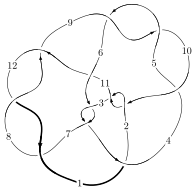
\includegraphics[width=112pt]{../../../GIT/diagram.site/Diagrams/png/2006_12a_1205.png}\\
\ \ \ A knot diagram\footnotemark}&
\allowdisplaybreaks
\textbf{Linearized knot diagam} \\
\cline{2-2}
 &
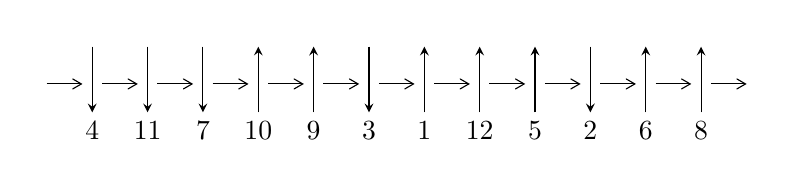
\begin{tikzpicture}[x=20pt, y=17pt]
	% nodes
	\node (C0) at (0, 0) {};
	\node (C1) at (1, 0) {};
	\node (C1U) at (1, +1) {};
	\node (C1D) at (1, -1) {4};

	\node (C2) at (2, 0) {};
	\node (C2U) at (2, +1) {};
	\node (C2D) at (2, -1) {11};

	\node (C3) at (3, 0) {};
	\node (C3U) at (3, +1) {};
	\node (C3D) at (3, -1) {7};

	\node (C4) at (4, 0) {};
	\node (C4U) at (4, +1) {};
	\node (C4D) at (4, -1) {10};

	\node (C5) at (5, 0) {};
	\node (C5U) at (5, +1) {};
	\node (C5D) at (5, -1) {9};

	\node (C6) at (6, 0) {};
	\node (C6U) at (6, +1) {};
	\node (C6D) at (6, -1) {3};

	\node (C7) at (7, 0) {};
	\node (C7U) at (7, +1) {};
	\node (C7D) at (7, -1) {1};

	\node (C8) at (8, 0) {};
	\node (C8U) at (8, +1) {};
	\node (C8D) at (8, -1) {12};

	\node (C9) at (9, 0) {};
	\node (C9U) at (9, +1) {};
	\node (C9D) at (9, -1) {5};

	\node (C10) at (10, 0) {};
	\node (C10U) at (10, +1) {};
	\node (C10D) at (10, -1) {2};

	\node (C11) at (11, 0) {};
	\node (C11U) at (11, +1) {};
	\node (C11D) at (11, -1) {6};

	\node (C12) at (12, 0) {};
	\node (C12U) at (12, +1) {};
	\node (C12D) at (12, -1) {8};
	\node (C13) at (13, 0) {};

	% arrows
	\draw[->,>={angle 60}]
	(C0) edge (C1) (C1) edge (C2) (C2) edge (C3) (C3) edge (C4) (C4) edge (C5) (C5) edge (C6) (C6) edge (C7) (C7) edge (C8) (C8) edge (C9) (C9) edge (C10) (C10) edge (C11) (C11) edge (C12) (C12) edge (C13) ;	\draw[->,>=stealth]
	(C1U) edge (C1D) (C2U) edge (C2D) (C3U) edge (C3D) (C4D) edge (C4U) (C5D) edge (C5U) (C6U) edge (C6D) (C7D) edge (C7U) (C8D) edge (C8U) (C9D) edge (C9U) (C10U) edge (C10D) (C11D) edge (C11U) (C12D) edge (C12U) ;
	\end{tikzpicture} \\
\hhline{~~} \\& 
\textbf{Solving Sequence} \\ \cline{2-2} 
 &
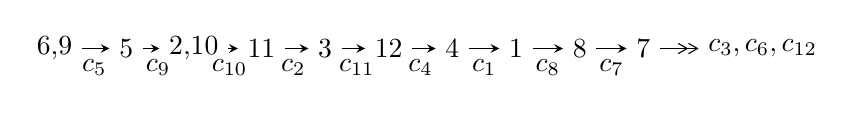
\begin{tikzpicture}[x=23pt, y=7pt]
	% node
	\node (A0) at (-1/8, 0) {6,9};
	\node (A1) at (1, 0) {5};
	\node (A2) at (33/16, 0) {2,10};
	\node (A3) at (25/8, 0) {11};
	\node (A4) at (33/8, 0) {3};
	\node (A5) at (41/8, 0) {12};
	\node (A6) at (49/8, 0) {4};
	\node (A7) at (57/8, 0) {1};
	\node (A8) at (65/8, 0) {8};
	\node (A9) at (73/8, 0) {7};
	\node (C1) at (1/2, -1) {$c_{5}$};
	\node (C2) at (3/2, -1) {$c_{9}$};
	\node (C3) at (21/8, -1) {$c_{10}$};
	\node (C4) at (29/8, -1) {$c_{2}$};
	\node (C5) at (37/8, -1) {$c_{11}$};
	\node (C6) at (45/8, -1) {$c_{4}$};
	\node (C7) at (53/8, -1) {$c_{1}$};
	\node (C8) at (61/8, -1) {$c_{8}$};
	\node (C9) at (69/8, -1) {$c_{7}$};
	\node (A10) at (11, 0) {$c_{3},c_{6},c_{12}$};

	% edge
	\draw[->,>=stealth]	
	(A0) edge (A1) (A1) edge (A2) (A2) edge (A3) (A3) edge (A4) (A4) edge (A5) (A5) edge (A6) (A6) edge (A7) (A7) edge (A8) (A8) edge (A9) ;
	\draw[->>,>={angle 60}]	
	(A9) edge (A10);
\end{tikzpicture} \\ 

\end{tabular} \\

\footnotetext{
The image of knot diagram is generated by the software ``\textbf{Draw programme}" developed by Andrew Bartholomew(\url{http://www.layer8.co.uk/maths/draw/index.htm\#Running-draw}), where we modified some parts for our purpose(\url{https://github.com/CATsTAILs/LinksPainter}).
}\phantom \\ \newline 
\centering \textbf{Ideals for irreducible components\footnotemark of $X_{\text{par}}$} 
 
\begin{align*}
I^u_{1}&=\langle 
73 u^{10}-18 u^9+462 u^8-140 u^7+1023 u^6-266 u^5+780 u^4+66 u^3+131 u^2+119 b+230 u+144,\\
\phantom{I^u_{1}}&\phantom{= \langle  }-209 u^{10}+120 u^9+\cdots+119 a-365,\;u^{11}+6 u^9+12 u^7+2 u^6+8 u^5+7 u^4+3 u^3+5 u^2+4 u+1\rangle \\
I^u_{2}&=\langle 
1.25318\times10^{92} u^{59}+2.44302\times10^{92} u^{58}+\cdots+8.16358\times10^{92} b-9.04940\times10^{93},\\
\phantom{I^u_{2}}&\phantom{= \langle  }-3.40806\times10^{92} u^{59}-3.96269\times10^{92} u^{58}+\cdots+4.08179\times10^{93} a+7.98134\times10^{94},\\
\phantom{I^u_{2}}&\phantom{= \langle  }u^{60}+2 u^{59}+\cdots-252 u+36\rangle \\
I^u_{3}&=\langle 
- a u+b- u+1,\;3 a^2-2 a u-2 a+u-2,\;u^2- u+1\rangle \\
I^u_{4}&=\langle 
- a u+b+2 a+1,\;6 a^2+3 a u+6 a+u+1,\;u^2+2\rangle \\
I^u_{5}&=\langle 
3 b+5 u+4,\;3 a+u-1,\;u^2+u+1\rangle \\
\\
I^v_{1}&=\langle 
a,\;3 b- v,\;v^2+3 v+3\rangle \\
\end{align*}
\raggedright * 6 irreducible components of $\dim_{\mathbb{C}}=0$, with total 83 representations.\\
\footnotetext{All coefficients of polynomials are rational numbers. But the coefficients are sometimes approximated in decimal forms when there is not enough margin.}
\newpage
\renewcommand{\arraystretch}{1}
\centering \section*{I. $I^u_{1}= \langle 73 u^{10}-18 u^9+\cdots+119 b+144,\;-209 u^{10}+120 u^9+\cdots+119 a-365,\;u^{11}+6 u^9+\cdots+4 u+1 \rangle$}
\flushleft \textbf{(i) Arc colorings}\\
\begin{tabular}{m{7pt} m{180pt} m{7pt} m{180pt} }
\flushright $a_{6}=$&$\begin{pmatrix}1\\0\end{pmatrix}$ \\
\flushright $a_{9}=$&$\begin{pmatrix}0\\u\end{pmatrix}$ \\
\flushright $a_{5}=$&$\begin{pmatrix}1\\u^2\end{pmatrix}$ \\
\flushright $a_{2}=$&$\begin{pmatrix}1.75630 u^{10}-1.00840 u^{9}+\cdots+7.21849 u+3.06723\\-0.613445 u^{10}+0.151261 u^{9}+\cdots-1.93277 u-1.21008\end{pmatrix}$ \\
\flushright $a_{10}=$&$\begin{pmatrix}u\\u^3+u\end{pmatrix}$ \\
\flushright $a_{11}=$&$\begin{pmatrix}0.815126 u^{10}-0.420168 u^{9}+\cdots+3.92437 u+1.36134\\-0.815126 u^{10}+0.420168 u^{9}+\cdots-3.92437 u-2.36134\end{pmatrix}$ \\
\flushright $a_{3}=$&$\begin{pmatrix}\frac{8}{7} u^{10}-\frac{6}{7} u^9+\cdots+\frac{37}{7} u+\frac{13}{7}\\\frac{9}{7} u^{10}-\frac{5}{7} u^9+\cdots+\frac{39}{7} u+\frac{19}{7}\end{pmatrix}$ \\
\flushright $a_{12}=$&$\begin{pmatrix}-1\\-0.815126 u^{10}+0.420168 u^{9}+\cdots-3.92437 u-2.36134\end{pmatrix}$ \\
\flushright $a_{4}=$&$\begin{pmatrix}u^2+1\\u^4+2 u^2\end{pmatrix}$ \\
\flushright $a_{1}=$&$\begin{pmatrix}- u^2-1\\-1.04202 u^{10}+0.722689 u^{9}+\cdots-4.78992 u-2.78151\end{pmatrix}$ \\
\flushright $a_{8}=$&$\begin{pmatrix}- u\\0.420168 u^{10}-0.226891 u^{9}+\cdots+1.89916 u+0.815126\end{pmatrix}$ \\
\flushright $a_{7}=$&$\begin{pmatrix}- u^3-2 u\\\frac{8}{7} u^{10}-\frac{6}{7} u^9+\cdots+\frac{23}{7} u+\frac{13}{7}\end{pmatrix}$\\&\end{tabular}
\flushleft \textbf{(ii) Obstruction class $= -1$}\\~\\
\flushleft \textbf{(iii) Cusp Shapes $= \frac{372}{119} u^{10}-\frac{20}{119} u^9+\frac{300}{17} u^8+\frac{8}{17} u^7+\frac{3596}{119} u^6+\frac{192}{17} u^5+\frac{1184}{119} u^4+\frac{3088}{119} u^3+\frac{172}{119} u^2+\frac{520}{119} u+\frac{1350}{119}$}\\~\\
\newpage\renewcommand{\arraystretch}{1}
\flushleft \textbf{(iv) u-Polynomials at the component}\newline \\
\begin{tabular}{m{50pt}|m{274pt}}
Crossings & \hspace{64pt}u-Polynomials at each crossing \\
\hline $$\begin{aligned}c_{1}\end{aligned}$$&$\begin{aligned}
&17(17 u^{11}-173 u^{10}+\cdots+236 u-40)
\end{aligned}$\\
\hline $$\begin{aligned}c_{2},c_{3},c_{6}\\c_{10}\end{aligned}$$&$\begin{aligned}
&u^{11}+2 u^{10}-2 u^9-6 u^8+4 u^6+2 u^5+5 u^4+7 u^3+3 u^2+1
\end{aligned}$\\
\hline $$\begin{aligned}c_{4},c_{5},c_{7}\\c_{8},c_{9},c_{12}\end{aligned}$$&$\begin{aligned}
&u^{11}+6 u^9+12 u^7-2 u^6+8 u^5-7 u^4+3 u^3-5 u^2+4 u-1
\end{aligned}$\\
\hline $$\begin{aligned}c_{11}\end{aligned}$$&$\begin{aligned}
&17(17 u^{11}-173 u^{10}+\cdots+1920 u-256)
\end{aligned}$\\
\hline
\end{tabular}\\~\\
\newpage\renewcommand{\arraystretch}{1}
\flushleft \textbf{(v) Riley Polynomials at the component}\newline \\
\begin{tabular}{m{50pt}|m{274pt}}
Crossings & \hspace{64pt}Riley Polynomials at each crossing \\
\hline $$\begin{aligned}c_{1}\end{aligned}$$&$\begin{aligned}
&289(289 y^{11}-4463 y^{10}+\cdots-8944 y-1600)
\end{aligned}$\\
\hline $$\begin{aligned}c_{2},c_{3},c_{6}\\c_{10}\end{aligned}$$&$\begin{aligned}
&y^{11}-8 y^{10}+\cdots-6 y-1
\end{aligned}$\\
\hline $$\begin{aligned}c_{4},c_{5},c_{7}\\c_{8},c_{9},c_{12}\end{aligned}$$&$\begin{aligned}
&y^{11}+12 y^{10}+\cdots+6 y-1
\end{aligned}$\\
\hline $$\begin{aligned}c_{11}\end{aligned}$$&$\begin{aligned}
&289(289 y^{11}+875 y^{10}+\cdots+311296 y-65536)
\end{aligned}$\\
\hline
\end{tabular}\\~\\
\newpage\flushleft \textbf{(vi) Complex Volumes and Cusp Shapes}
$$\begin{array}{c|c|c}  
\text{Solutions to }I^u_{1}& \I (\text{vol} + \sqrt{-1}CS) & \text{Cusp shape}\\
 \hline 
\begin{aligned}
u &= \phantom{-}0.680975 + 0.675052 I \\
a &= \phantom{-}0.702616 - 0.178305 I \\
b &= \phantom{-}0.09896 + 1.78843 I\end{aligned}
 & -7.07216 + 7.70619 I & -4.42118 - 7.71824 I \\ \hline\begin{aligned}
u &= \phantom{-}0.680975 - 0.675052 I \\
a &= \phantom{-}0.702616 + 0.178305 I \\
b &= \phantom{-}0.09896 - 1.78843 I\end{aligned}
 & -7.07216 - 7.70619 I & -4.42118 + 7.71824 I \\ \hline\begin{aligned}
u &= \phantom{-}0.161381 + 1.138270 I \\
a &= \phantom{-}0.151626 - 0.748852 I \\
b &= -0.166833 - 0.455380 I\end{aligned}
 & -4.56283 + 4.40440 I & -3.38740 - 7.31700 I \\ \hline\begin{aligned}
u &= \phantom{-}0.161381 - 1.138270 I \\
a &= \phantom{-}0.151626 + 0.748852 I \\
b &= -0.166833 + 0.455380 I\end{aligned}
 & -4.56283 - 4.40440 I & -3.38740 + 7.31700 I \\ \hline\begin{aligned}
u &= -0.441939 + 0.225736 I \\
a &= -0.875079 + 0.513848 I \\
b &= -0.189711 + 0.169501 I\end{aligned}
 & \phantom{-}0.884913 - 0.517986 I & \phantom{-}8.70917 + 3.40201 I \\ \hline\begin{aligned}
u &= -0.441939 - 0.225736 I \\
a &= -0.875079 - 0.513848 I \\
b &= -0.189711 - 0.169501 I\end{aligned}
 & \phantom{-}0.884913 + 0.517986 I & \phantom{-}8.70917 - 3.40201 I \\ \hline\begin{aligned}
u &= -0.490964\phantom{ +0.000000I} \\
a &= \phantom{-}1.13114\phantom{ +0.000000I} \\
b &= -1.04783\phantom{ +0.000000I}\end{aligned}
 & -4.15298\phantom{ +0.000000I} & \phantom{-}7.21490\phantom{ +0.000000I} \\ \hline\begin{aligned}
u &= \phantom{-}0.14545 + 1.56334 I \\
a &= -0.406442 - 0.035002 I \\
b &= \phantom{-}1.119140 + 0.082033 I\end{aligned}
 & -11.62950 + 4.58145 I & -3.17899 - 3.55621 I \\ \hline\begin{aligned}
u &= \phantom{-}0.14545 - 1.56334 I \\
a &= -0.406442 + 0.035002 I \\
b &= \phantom{-}1.119140 - 0.082033 I\end{aligned}
 & -11.62950 - 4.58145 I & -3.17899 + 3.55621 I \\ \hline\begin{aligned}
u &= -0.30038 + 1.63421 I \\
a &= -0.72653 - 2.10196 I \\
b &= -0.74940 + 3.07893 I\end{aligned}
 & \phantom{-}17.0539 - 15.5687 I & -8.09374 + 6.58975 I\\
 \hline 
 \end{array}$$\newpage$$\begin{array}{c|c|c}  
\text{Solutions to }I^u_{1}& \I (\text{vol} + \sqrt{-1}CS) & \text{Cusp shape}\\
 \hline 
\begin{aligned}
u &= -0.30038 - 1.63421 I \\
a &= -0.72653 + 2.10196 I \\
b &= -0.74940 - 3.07893 I\end{aligned}
 & \phantom{-}17.0539 + 15.5687 I & -8.09374 - 6.58975 I\\
 \hline 
 \end{array}$$\newpage\newpage\renewcommand{\arraystretch}{1}
\centering \section*{II. $I^u_{2}= \langle 1.25\times10^{92} u^{59}+2.44\times10^{92} u^{58}+\cdots+8.16\times10^{92} b-9.05\times10^{93},\;-3.41\times10^{92} u^{59}-3.96\times10^{92} u^{58}+\cdots+4.08\times10^{93} a+7.98\times10^{94},\;u^{60}+2 u^{59}+\cdots-252 u+36 \rangle$}
\flushleft \textbf{(i) Arc colorings}\\
\begin{tabular}{m{7pt} m{180pt} m{7pt} m{180pt} }
\flushright $a_{6}=$&$\begin{pmatrix}1\\0\end{pmatrix}$ \\
\flushright $a_{9}=$&$\begin{pmatrix}0\\u\end{pmatrix}$ \\
\flushright $a_{5}=$&$\begin{pmatrix}1\\u^2\end{pmatrix}$ \\
\flushright $a_{2}=$&$\begin{pmatrix}0.0834942 u^{59}+0.0970821 u^{58}+\cdots+113.120 u-19.5535\\-0.153508 u^{59}-0.299258 u^{58}+\cdots-77.5361 u+11.0851\end{pmatrix}$ \\
\flushright $a_{10}=$&$\begin{pmatrix}u\\u^3+u\end{pmatrix}$ \\
\flushright $a_{11}=$&$\begin{pmatrix}0.200490 u^{59}+0.427440 u^{58}+\cdots+66.0395 u-10.3644\\-0.0334245 u^{59}-0.0366283 u^{58}+\cdots-43.3403 u+8.64055\end{pmatrix}$ \\
\flushright $a_{3}=$&$\begin{pmatrix}-0.114742 u^{59}-0.326177 u^{58}+\cdots+10.2529 u-5.95573\\-0.0790482 u^{59}-0.144541 u^{58}+\cdots-49.6201 u+7.70720\end{pmatrix}$ \\
\flushright $a_{12}=$&$\begin{pmatrix}0.167066 u^{59}+0.390811 u^{58}+\cdots+22.6992 u-1.72388\\-0.0334245 u^{59}-0.0366283 u^{58}+\cdots-43.3403 u+8.64055\end{pmatrix}$ \\
\flushright $a_{4}=$&$\begin{pmatrix}u^2+1\\u^4+2 u^2\end{pmatrix}$ \\
\flushright $a_{1}=$&$\begin{pmatrix}0.0413371 u^{59}+0.0216303 u^{58}+\cdots+86.0346 u-13.9193\\-0.120341 u^{59}-0.219185 u^{58}+\cdots-70.0325 u+10.5469\end{pmatrix}$ \\
\flushright $a_{8}=$&$\begin{pmatrix}0.0796060 u^{59}+0.168470 u^{58}+\cdots+8.25556 u+4.31633\\-0.0126674 u^{59}-0.0693921 u^{58}+\cdots+26.9172 u-3.41367\end{pmatrix}$ \\
\flushright $a_{7}=$&$\begin{pmatrix}0.0484754 u^{59}+0.174481 u^{58}+\cdots-39.6371 u+10.1820\\-0.0492349 u^{59}-0.128310 u^{58}+\cdots-11.5918 u+1.43518\end{pmatrix}$\\&\end{tabular}
\flushleft \textbf{(ii) Obstruction class $= -1$}\\~\\
\flushleft \textbf{(iii) Cusp Shapes $= 0.349952 u^{59}+0.763128 u^{58}+\cdots+53.7078 u-5.40438$}\\~\\
\newpage\renewcommand{\arraystretch}{1}
\flushleft \textbf{(iv) u-Polynomials at the component}\newline \\
\begin{tabular}{m{50pt}|m{274pt}}
Crossings & \hspace{64pt}u-Polynomials at each crossing \\
\hline $$\begin{aligned}c_{1}\end{aligned}$$&$\begin{aligned}
&9(3 u^{30}+14 u^{29}+\cdots+1087 u-223)^{2}
\end{aligned}$\\
\hline $$\begin{aligned}c_{2},c_{3},c_{6}\\c_{10}\end{aligned}$$&$\begin{aligned}
&u^{60}+4 u^{59}+\cdots+649 u+171
\end{aligned}$\\
\hline $$\begin{aligned}c_{4},c_{5},c_{7}\\c_{8},c_{9},c_{12}\end{aligned}$$&$\begin{aligned}
&u^{60}-2 u^{59}+\cdots+252 u+36
\end{aligned}$\\
\hline $$\begin{aligned}c_{11}\end{aligned}$$&$\begin{aligned}
&9(3 u^{30}+10 u^{29}+\cdots+1366 u+167)^{2}
\end{aligned}$\\
\hline
\end{tabular}\\~\\
\newpage\renewcommand{\arraystretch}{1}
\flushleft \textbf{(v) Riley Polynomials at the component}\newline \\
\begin{tabular}{m{50pt}|m{274pt}}
Crossings & \hspace{64pt}Riley Polynomials at each crossing \\
\hline $$\begin{aligned}c_{1}\end{aligned}$$&$\begin{aligned}
&81(9 y^{30}-274 y^{29}+\cdots-2522245 y+49729)^{2}
\end{aligned}$\\
\hline $$\begin{aligned}c_{2},c_{3},c_{6}\\c_{10}\end{aligned}$$&$\begin{aligned}
&y^{60}-48 y^{59}+\cdots-61075 y+29241
\end{aligned}$\\
\hline $$\begin{aligned}c_{4},c_{5},c_{7}\\c_{8},c_{9},c_{12}\end{aligned}$$&$\begin{aligned}
&y^{60}+66 y^{59}+\cdots+27792 y+1296
\end{aligned}$\\
\hline $$\begin{aligned}c_{11}\end{aligned}$$&$\begin{aligned}
&81(9 y^{30}+218 y^{29}+\cdots+161758 y+27889)^{2}
\end{aligned}$\\
\hline
\end{tabular}\\~\\
\newpage\flushleft \textbf{(vi) Complex Volumes and Cusp Shapes}
$$\begin{array}{c|c|c}  
\text{Solutions to }I^u_{2}& \I (\text{vol} + \sqrt{-1}CS) & \text{Cusp shape}\\
 \hline 
\begin{aligned}
u &= -0.759750 + 0.662027 I \\
a &= -0.931053 + 0.172845 I \\
b &= -0.09008 + 1.98013 I\end{aligned}
 & -1.86631 - 2.71902 I & \phantom{-0.000000 } 0 \\ \hline\begin{aligned}
u &= -0.759750 - 0.662027 I \\
a &= -0.931053 - 0.172845 I \\
b &= -0.09008 - 1.98013 I\end{aligned}
 & -1.86631 + 2.71902 I & \phantom{-0.000000 } 0 \\ \hline\begin{aligned}
u &= -0.314512 + 0.960641 I \\
a &= -0.190977 + 0.499858 I \\
b &= \phantom{-}0.419438 + 0.858326 I\end{aligned}
 & -1.10026 - 2.27454 I & \phantom{-0.000000 } 0 \\ \hline\begin{aligned}
u &= -0.314512 - 0.960641 I \\
a &= -0.190977 - 0.499858 I \\
b &= \phantom{-}0.419438 - 0.858326 I\end{aligned}
 & -1.10026 + 2.27454 I & \phantom{-0.000000 } 0 \\ \hline\begin{aligned}
u &= -0.129337 + 0.950966 I \\
a &= -1.60981 - 1.06801 I \\
b &= \phantom{-}0.20747 + 1.44586 I\end{aligned}
 & -12.50500 - 0.66605 I & -8.84093 + 0. I\phantom{ +0.000000I} \\ \hline\begin{aligned}
u &= -0.129337 - 0.950966 I \\
a &= -1.60981 + 1.06801 I \\
b &= \phantom{-}0.20747 - 1.44586 I\end{aligned}
 & -12.50500 + 0.66605 I & -8.84093 + 0. I\phantom{ +0.000000I} \\ \hline\begin{aligned}
u &= -0.588192 + 0.683594 I \\
a &= \phantom{-}1.039310 - 0.418609 I \\
b &= -0.102741 - 0.312706 I\end{aligned}
 & -9.38994 - 6.05319 I & -4.32641 + 5.70687 I \\ \hline\begin{aligned}
u &= -0.588192 - 0.683594 I \\
a &= \phantom{-}1.039310 + 0.418609 I \\
b &= -0.102741 + 0.312706 I\end{aligned}
 & -9.38994 + 6.05319 I & -4.32641 - 5.70687 I \\ \hline\begin{aligned}
u &= \phantom{-}0.776674 + 0.411211 I \\
a &= \phantom{-}1.206490 + 0.140254 I \\
b &= \phantom{-}0.23920 + 1.51841 I\end{aligned}
 & -6.21939 - 2.80157 I & -5.28737 + 3.00592 I \\ \hline\begin{aligned}
u &= \phantom{-}0.776674 - 0.411211 I \\
a &= \phantom{-}1.206490 - 0.140254 I \\
b &= \phantom{-}0.23920 - 1.51841 I\end{aligned}
 & -6.21939 + 2.80157 I & -5.28737 - 3.00592 I\\
 \hline 
 \end{array}$$\newpage$$\begin{array}{c|c|c}  
\text{Solutions to }I^u_{2}& \I (\text{vol} + \sqrt{-1}CS) & \text{Cusp shape}\\
 \hline 
\begin{aligned}
u &= -0.916850 + 0.719386 I \\
a &= \phantom{-}0.816528 - 0.325861 I \\
b &= -0.10977 - 2.54265 I\end{aligned}
 & -14.6835 - 11.0154 I & \phantom{-0.000000 } 0 \\ \hline\begin{aligned}
u &= -0.916850 - 0.719386 I \\
a &= \phantom{-}0.816528 + 0.325861 I \\
b &= -0.10977 + 2.54265 I\end{aligned}
 & -14.6835 + 11.0154 I & \phantom{-0.000000 } 0 \\ \hline\begin{aligned}
u &= \phantom{-}0.576968 + 0.560729 I \\
a &= -0.802985 - 0.539725 I \\
b &= -0.221236 - 0.702999 I\end{aligned}
 & -4.48267 + 2.06711 I & \phantom{-}1.19955 - 3.78893 I \\ \hline\begin{aligned}
u &= \phantom{-}0.576968 - 0.560729 I \\
a &= -0.802985 + 0.539725 I \\
b &= -0.221236 + 0.702999 I\end{aligned}
 & -4.48267 - 2.06711 I & \phantom{-}1.19955 + 3.78893 I \\ \hline\begin{aligned}
u &= -0.355589 + 0.707290 I \\
a &= -0.035366 + 0.978857 I \\
b &= \phantom{-}0.126483 - 1.162340 I\end{aligned}
 & -6.21939 - 2.80157 I & -5.28737 + 3.00592 I \\ \hline\begin{aligned}
u &= -0.355589 - 0.707290 I \\
a &= -0.035366 - 0.978857 I \\
b &= \phantom{-}0.126483 + 1.162340 I\end{aligned}
 & -6.21939 + 2.80157 I & -5.28737 - 3.00592 I \\ \hline\begin{aligned}
u &= -1.076620 + 0.557141 I \\
a &= \phantom{-}1.321450 - 0.193835 I \\
b &= \phantom{-}1.09050 - 2.33731 I\end{aligned}
 & -14.0759 + 4.5063 I & \phantom{-0.000000 } 0 \\ \hline\begin{aligned}
u &= -1.076620 - 0.557141 I \\
a &= \phantom{-}1.321450 + 0.193835 I \\
b &= \phantom{-}1.09050 + 2.33731 I\end{aligned}
 & -14.0759 - 4.5063 I & \phantom{-0.000000 } 0 \\ \hline\begin{aligned}
u &= -0.646640 + 0.296075 I \\
a &= \phantom{-}0.016407 - 0.488252 I \\
b &= \phantom{-}0.682960 - 1.103020 I\end{aligned}
 & -8.24661 + 1.82485 I & -1.78640 - 0.62717 I \\ \hline\begin{aligned}
u &= -0.646640 - 0.296075 I \\
a &= \phantom{-}0.016407 + 0.488252 I \\
b &= \phantom{-}0.682960 + 1.103020 I\end{aligned}
 & -8.24661 - 1.82485 I & -1.78640 + 0.62717 I\\
 \hline 
 \end{array}$$\newpage$$\begin{array}{c|c|c}  
\text{Solutions to }I^u_{2}& \I (\text{vol} + \sqrt{-1}CS) & \text{Cusp shape}\\
 \hline 
\begin{aligned}
u &= \phantom{-}0.278410 + 1.260600 I \\
a &= -0.247426 - 0.743643 I \\
b &= \phantom{-}1.277450 - 0.383957 I\end{aligned}
 & -4.84465\phantom{ +0.000000I} & \phantom{-0.000000 } 0 \\ \hline\begin{aligned}
u &= \phantom{-}0.278410 - 1.260600 I \\
a &= -0.247426 + 0.743643 I \\
b &= \phantom{-}1.277450 + 0.383957 I\end{aligned}
 & -4.84465\phantom{ +0.000000I} & \phantom{-0.000000 } 0 \\ \hline\begin{aligned}
u &= \phantom{-}1.092800 + 0.750740 I \\
a &= -1.124120 - 0.436933 I \\
b &= -0.32876 - 3.19706 I\end{aligned}
 & -8.92368 + 3.64409 I & \phantom{-0.000000 } 0 \\ \hline\begin{aligned}
u &= \phantom{-}1.092800 - 0.750740 I \\
a &= -1.124120 + 0.436933 I \\
b &= -0.32876 + 3.19706 I\end{aligned}
 & -8.92368 - 3.64409 I & \phantom{-0.000000 } 0 \\ \hline\begin{aligned}
u &= \phantom{-}0.06050 + 1.41516 I \\
a &= \phantom{-}1.40096 + 0.56694 I \\
b &= -1.56146 - 0.59391 I\end{aligned}
 & -7.20542 + 0.22364 I & \phantom{-0.000000 } 0 \\ \hline\begin{aligned}
u &= \phantom{-}0.06050 - 1.41516 I \\
a &= \phantom{-}1.40096 - 0.56694 I \\
b &= -1.56146 + 0.59391 I\end{aligned}
 & -7.20542 - 0.22364 I & \phantom{-0.000000 } 0 \\ \hline\begin{aligned}
u &= -0.06398 + 1.43597 I \\
a &= -0.171576 - 0.010774 I \\
b &= \phantom{-}0.742412 - 0.071303 I\end{aligned}
 & -4.48267 - 2.06711 I & \phantom{-0.000000 } 0 \\ \hline\begin{aligned}
u &= -0.06398 - 1.43597 I \\
a &= -0.171576 + 0.010774 I \\
b &= \phantom{-}0.742412 + 0.071303 I\end{aligned}
 & -4.48267 + 2.06711 I & \phantom{-0.000000 } 0 \\ \hline\begin{aligned}
u &= \phantom{-}0.225772 + 0.478556 I \\
a &= \phantom{-}2.00278 + 0.98084 I \\
b &= -0.296782 + 0.092033 I\end{aligned}
 & -1.86631 + 2.71902 I & -6.02392 - 8.48187 I \\ \hline\begin{aligned}
u &= \phantom{-}0.225772 - 0.478556 I \\
a &= \phantom{-}2.00278 - 0.98084 I \\
b &= -0.296782 - 0.092033 I\end{aligned}
 & -1.86631 - 2.71902 I & -6.02392 + 8.48187 I\\
 \hline 
 \end{array}$$\newpage$$\begin{array}{c|c|c}  
\text{Solutions to }I^u_{2}& \I (\text{vol} + \sqrt{-1}CS) & \text{Cusp shape}\\
 \hline 
\begin{aligned}
u &= -0.05387 + 1.52215 I \\
a &= \phantom{-}2.31103 + 0.70700 I \\
b &= -3.18172 - 0.73741 I\end{aligned}
 & -13.6864\phantom{ +0.000000I} & \phantom{-0.000000 } 0 \\ \hline\begin{aligned}
u &= -0.05387 - 1.52215 I \\
a &= \phantom{-}2.31103 - 0.70700 I \\
b &= -3.18172 + 0.73741 I\end{aligned}
 & -13.6864\phantom{ +0.000000I} & \phantom{-0.000000 } 0 \\ \hline\begin{aligned}
u &= \phantom{-}0.05204 + 1.52292 I \\
a &= \phantom{-}0.65459 - 2.51222 I \\
b &= -0.60287 + 2.55575 I\end{aligned}
 & -8.24661 + 1.82485 I & \phantom{-0.000000 } 0 \\ \hline\begin{aligned}
u &= \phantom{-}0.05204 - 1.52292 I \\
a &= \phantom{-}0.65459 + 2.51222 I \\
b &= -0.60287 - 2.55575 I\end{aligned}
 & -8.24661 - 1.82485 I & \phantom{-0.000000 } 0 \\ \hline\begin{aligned}
u &= \phantom{-}0.18810 + 1.51588 I \\
a &= -0.87884 + 2.25051 I \\
b &= -0.27333 - 2.47353 I\end{aligned}
 & -12.50500 + 0.66605 I & \phantom{-0.000000 } 0 \\ \hline\begin{aligned}
u &= \phantom{-}0.18810 - 1.51588 I \\
a &= -0.87884 - 2.25051 I \\
b &= -0.27333 + 2.47353 I\end{aligned}
 & -12.50500 - 0.66605 I & \phantom{-0.000000 } 0 \\ \hline\begin{aligned}
u &= \phantom{-}0.244643 + 0.402854 I \\
a &= -0.334643 + 1.093090 I \\
b &= \phantom{-}0.256864 - 1.075110 I\end{aligned}
 & -1.70488 + 0.85900 I & -3.09812 + 2.75630 I \\ \hline\begin{aligned}
u &= \phantom{-}0.244643 - 0.402854 I \\
a &= -0.334643 - 1.093090 I \\
b &= \phantom{-}0.256864 + 1.075110 I\end{aligned}
 & -1.70488 - 0.85900 I & -3.09812 - 2.75630 I \\ \hline\begin{aligned}
u &= \phantom{-}0.05319 + 1.56037 I \\
a &= -0.242202 - 0.185041 I \\
b &= -0.623485 + 0.111421 I\end{aligned}
 & -8.92368 + 3.64409 I & \phantom{-0.000000 } 0 \\ \hline\begin{aligned}
u &= \phantom{-}0.05319 - 1.56037 I \\
a &= -0.242202 + 0.185041 I \\
b &= -0.623485 - 0.111421 I\end{aligned}
 & -8.92368 - 3.64409 I & \phantom{-0.000000 } 0\\
 \hline 
 \end{array}$$\newpage$$\begin{array}{c|c|c}  
\text{Solutions to }I^u_{2}& \I (\text{vol} + \sqrt{-1}CS) & \text{Cusp shape}\\
 \hline 
\begin{aligned}
u &= \phantom{-}0.045280 + 0.430914 I \\
a &= \phantom{-}2.09252 - 1.08737 I \\
b &= \phantom{-}1.15217 + 1.56271 I\end{aligned}
 & -7.20542 + 0.22364 I & -9.04537 + 1.25928 I \\ \hline\begin{aligned}
u &= \phantom{-}0.045280 - 0.430914 I \\
a &= \phantom{-}2.09252 + 1.08737 I \\
b &= \phantom{-}1.15217 - 1.56271 I\end{aligned}
 & -7.20542 - 0.22364 I & -9.04537 - 1.25928 I \\ \hline\begin{aligned}
u &= \phantom{-}0.264001 + 0.331764 I \\
a &= -0.075640 + 0.209812 I \\
b &= \phantom{-}0.785454 + 0.369858 I\end{aligned}
 & -1.70488 - 0.85900 I & -3.09812 - 2.75630 I \\ \hline\begin{aligned}
u &= \phantom{-}0.264001 - 0.331764 I \\
a &= -0.075640 - 0.209812 I \\
b &= \phantom{-}0.785454 - 0.369858 I\end{aligned}
 & -1.70488 + 0.85900 I & -3.09812 + 2.75630 I \\ \hline\begin{aligned}
u &= \phantom{-}0.415346 + 0.011561 I \\
a &= -1.51548 + 1.51134 I \\
b &= -0.315561 + 0.009208 I\end{aligned}
 & -1.10026 + 2.27454 I & \phantom{-}6.39783 - 4.86989 I \\ \hline\begin{aligned}
u &= \phantom{-}0.415346 - 0.011561 I \\
a &= -1.51548 - 1.51134 I \\
b &= -0.315561 - 0.009208 I\end{aligned}
 & -1.10026 - 2.27454 I & \phantom{-}6.39783 + 4.86989 I \\ \hline\begin{aligned}
u &= -0.19401 + 1.58701 I \\
a &= \phantom{-}0.49148 + 2.16389 I \\
b &= \phantom{-}0.52046 - 2.62595 I\end{aligned}
 & -9.38994 - 6.05319 I & \phantom{-0.000000 } 0 \\ \hline\begin{aligned}
u &= -0.19401 - 1.58701 I \\
a &= \phantom{-}0.49148 - 2.16389 I \\
b &= \phantom{-}0.52046 + 2.62595 I\end{aligned}
 & -9.38994 + 6.05319 I & \phantom{-0.000000 } 0 \\ \hline\begin{aligned}
u &= -0.10187 + 1.60028 I \\
a &= -0.36353 - 1.96711 I \\
b &= \phantom{-}0.25135 + 2.10282 I\end{aligned}
 & -14.0759 - 4.5063 I & \phantom{-0.000000 } 0 \\ \hline\begin{aligned}
u &= -0.10187 - 1.60028 I \\
a &= -0.36353 + 1.96711 I \\
b &= \phantom{-}0.25135 - 2.10282 I\end{aligned}
 & -14.0759 + 4.5063 I & \phantom{-0.000000 } 0\\
 \hline 
 \end{array}$$\newpage$$\begin{array}{c|c|c}  
\text{Solutions to }I^u_{2}& \I (\text{vol} + \sqrt{-1}CS) & \text{Cusp shape}\\
 \hline 
\begin{aligned}
u &= -0.17637 + 1.60289 I \\
a &= \phantom{-}0.015923 + 0.384340 I \\
b &= -0.632206 - 0.409488 I\end{aligned}
 & -17.1000 - 8.9031 I & \phantom{-0.000000 } 0 \\ \hline\begin{aligned}
u &= -0.17637 - 1.60289 I \\
a &= \phantom{-}0.015923 - 0.384340 I \\
b &= -0.632206 + 0.409488 I\end{aligned}
 & -17.1000 + 8.9031 I & \phantom{-0.000000 } 0 \\ \hline\begin{aligned}
u &= \phantom{-}0.20940 + 1.60061 I \\
a &= -0.54658 + 2.10296 I \\
b &= -0.36822 - 2.53572 I\end{aligned}
 & -14.6835 + 11.0154 I & \phantom{-0.000000 } 0 \\ \hline\begin{aligned}
u &= \phantom{-}0.20940 - 1.60061 I \\
a &= -0.54658 - 2.10296 I \\
b &= -0.36822 + 2.53572 I\end{aligned}
 & -14.6835 - 11.0154 I & \phantom{-0.000000 } 0 \\ \hline\begin{aligned}
u &= -0.02241 + 1.64609 I \\
a &= -0.32821 + 1.68373 I \\
b &= \phantom{-}1.15247 - 1.88578 I\end{aligned}
 & \phantom{-}18.0731 - 1.1594 I & \phantom{-0.000000 } 0 \\ \hline\begin{aligned}
u &= -0.02241 - 1.64609 I \\
a &= -0.32821 - 1.68373 I \\
b &= \phantom{-}1.15247 + 1.88578 I\end{aligned}
 & \phantom{-}18.0731 + 1.1594 I & \phantom{-0.000000 } 0 \\ \hline\begin{aligned}
u &= \phantom{-}0.31119 + 1.69477 I \\
a &= \phantom{-}0.41080 - 2.03463 I \\
b &= \phantom{-}1.37332 + 3.18776 I\end{aligned}
 & -17.1000 + 8.9031 I & \phantom{-0.000000 } 0 \\ \hline\begin{aligned}
u &= \phantom{-}0.31119 - 1.69477 I \\
a &= \phantom{-}0.41080 + 2.03463 I \\
b &= \phantom{-}1.37332 - 3.18776 I\end{aligned}
 & -17.1000 - 8.9031 I & \phantom{-0.000000 } 0 \\ \hline\begin{aligned}
u &= -0.39432 + 1.69567 I \\
a &= -0.21517 - 1.69581 I \\
b &= -2.06977 + 2.35462 I\end{aligned}
 & \phantom{-}18.0731 - 1.1594 I & \phantom{-0.000000 } 0 \\ \hline\begin{aligned}
u &= -0.39432 - 1.69567 I \\
a &= -0.21517 + 1.69581 I \\
b &= -2.06977 - 2.35462 I\end{aligned}
 & \phantom{-}18.0731 + 1.1594 I & \phantom{-0.000000 } 0\\
 \hline 
 \end{array}$$\newpage\newpage\renewcommand{\arraystretch}{1}
\centering \section*{III. $I^u_{3}= \langle - a u+b- u+1,\;3 a^2-2 a u-2 a+u-2,\;u^2- u+1 \rangle$}
\flushleft \textbf{(i) Arc colorings}\\
\begin{tabular}{m{7pt} m{180pt} m{7pt} m{180pt} }
\flushright $a_{6}=$&$\begin{pmatrix}1\\0\end{pmatrix}$ \\
\flushright $a_{9}=$&$\begin{pmatrix}0\\u\end{pmatrix}$ \\
\flushright $a_{5}=$&$\begin{pmatrix}1\\u-1\end{pmatrix}$ \\
\flushright $a_{2}=$&$\begin{pmatrix}a\\a u+u-1\end{pmatrix}$ \\
\flushright $a_{10}=$&$\begin{pmatrix}u\\u-1\end{pmatrix}$ \\
\flushright $a_{11}=$&$\begin{pmatrix}- a+u\\- a u\end{pmatrix}$ \\
\flushright $a_{3}=$&$\begin{pmatrix}u\\u-1\end{pmatrix}$ \\
\flushright $a_{12}=$&$\begin{pmatrix}- a u- a+u\\- a u\end{pmatrix}$ \\
\flushright $a_{4}=$&$\begin{pmatrix}u\\u-2\end{pmatrix}$ \\
\flushright $a_{1}=$&$\begin{pmatrix}a u+a- u\\2 a u-2 a+1\end{pmatrix}$ \\
\flushright $a_{8}=$&$\begin{pmatrix}-2 u+2\\a+1\end{pmatrix}$ \\
\flushright $a_{7}=$&$\begin{pmatrix}0\\- u\end{pmatrix}$\\&\end{tabular}
\flushleft \textbf{(ii) Obstruction class $= 1$}\\~\\
\flushleft \textbf{(iii) Cusp Shapes $= -4 u-4$}\\~\\
\newpage\renewcommand{\arraystretch}{1}
\flushleft \textbf{(iv) u-Polynomials at the component}\newline \\
\begin{tabular}{m{50pt}|m{274pt}}
Crossings & \hspace{64pt}u-Polynomials at each crossing \\
\hline $$\begin{aligned}c_{1}\end{aligned}$$&$\begin{aligned}
&3(3 u^4-6 u^3+u^2+2 u+1)
\end{aligned}$\\
\hline $$\begin{aligned}c_{2}\end{aligned}$$&$\begin{aligned}
&(u-1)^4
\end{aligned}$\\
\hline $$\begin{aligned}c_{3},c_{4},c_{5}\end{aligned}$$&$\begin{aligned}
&(u^2- u+1)^2
\end{aligned}$\\
\hline $$\begin{aligned}c_{6},c_{9}\end{aligned}$$&$\begin{aligned}
&(u^2+u+1)^2
\end{aligned}$\\
\hline $$\begin{aligned}c_{7},c_{8},c_{12}\end{aligned}$$&$\begin{aligned}
&(u^2+2)^2
\end{aligned}$\\
\hline $$\begin{aligned}c_{10}\end{aligned}$$&$\begin{aligned}
&(u+1)^4
\end{aligned}$\\
\hline $$\begin{aligned}c_{11}\end{aligned}$$&$\begin{aligned}
&3(3 u^4+4 u^2+4 u+1)
\end{aligned}$\\
\hline
\end{tabular}\\~\\
\newpage\renewcommand{\arraystretch}{1}
\flushleft \textbf{(v) Riley Polynomials at the component}\newline \\
\begin{tabular}{m{50pt}|m{274pt}}
Crossings & \hspace{64pt}Riley Polynomials at each crossing \\
\hline $$\begin{aligned}c_{1}\end{aligned}$$&$\begin{aligned}
&9(9 y^4-30 y^3+31 y^2-2 y+1)
\end{aligned}$\\
\hline $$\begin{aligned}c_{2},c_{10}\end{aligned}$$&$\begin{aligned}
&(y-1)^4
\end{aligned}$\\
\hline $$\begin{aligned}c_{3},c_{4},c_{5}\\c_{6},c_{9}\end{aligned}$$&$\begin{aligned}
&(y^2+y+1)^2
\end{aligned}$\\
\hline $$\begin{aligned}c_{7},c_{8},c_{12}\end{aligned}$$&$\begin{aligned}
&(y+2)^4
\end{aligned}$\\
\hline $$\begin{aligned}c_{11}\end{aligned}$$&$\begin{aligned}
&9(9 y^4+24 y^3+22 y^2-8 y+1)
\end{aligned}$\\
\hline
\end{tabular}\\~\\
\newpage\flushleft \textbf{(vi) Complex Volumes and Cusp Shapes}
$$\begin{array}{c|c|c}  
\text{Solutions to }I^u_{3}& \I (\text{vol} + \sqrt{-1}CS) & \text{Cusp shape}\\
 \hline 
\begin{aligned}
u &= \phantom{-}0.500000 + 0.866025 I \\
a &= \phantom{-}1.316500 + 0.288675 I \\
b &= -0.09175 + 2.15048 I\end{aligned}
 & -6.57974 + 2.02988 I & -6.00000 - 3.46410 I \\ \hline\begin{aligned}
u &= \phantom{-}0.500000 + 0.866025 I \\
a &= -0.316497 + 0.288675 I \\
b &= -0.908248 + 0.736269 I\end{aligned}
 & -6.57974 + 2.02988 I & -6.00000 - 3.46410 I \\ \hline\begin{aligned}
u &= \phantom{-}0.500000 - 0.866025 I \\
a &= \phantom{-}1.316500 - 0.288675 I \\
b &= -0.09175 - 2.15048 I\end{aligned}
 & -6.57974 - 2.02988 I & -6.00000 + 3.46410 I \\ \hline\begin{aligned}
u &= \phantom{-}0.500000 - 0.866025 I \\
a &= -0.316497 - 0.288675 I \\
b &= -0.908248 - 0.736269 I\end{aligned}
 & -6.57974 - 2.02988 I & -6.00000 + 3.46410 I\\
 \hline 
 \end{array}$$\newpage\newpage\renewcommand{\arraystretch}{1}
\centering \section*{IV. $I^u_{4}= \langle - a u+b+2 a+1,\;6 a^2+3 a u+6 a+u+1,\;u^2+2 \rangle$}
\flushleft \textbf{(i) Arc colorings}\\
\begin{tabular}{m{7pt} m{180pt} m{7pt} m{180pt} }
\flushright $a_{6}=$&$\begin{pmatrix}1\\0\end{pmatrix}$ \\
\flushright $a_{9}=$&$\begin{pmatrix}0\\u\end{pmatrix}$ \\
\flushright $a_{5}=$&$\begin{pmatrix}1\\-2\end{pmatrix}$ \\
\flushright $a_{2}=$&$\begin{pmatrix}a\\a u-2 a-1\end{pmatrix}$ \\
\flushright $a_{10}=$&$\begin{pmatrix}u\\- u\end{pmatrix}$ \\
\flushright $a_{11}=$&$\begin{pmatrix}a u+a+\frac{3}{2} u\\-2 a- u-1\end{pmatrix}$ \\
\flushright $a_{3}=$&$\begin{pmatrix}a u- a-\frac{1}{2} u-2\\1\end{pmatrix}$ \\
\flushright $a_{12}=$&$\begin{pmatrix}a u- a+\frac{1}{2} u-1\\-2 a- u-1\end{pmatrix}$ \\
\flushright $a_{4}=$&$\begin{pmatrix}-1\\0\end{pmatrix}$ \\
\flushright $a_{1}=$&$\begin{pmatrix}a u- a-1\\a u-2 a-1\end{pmatrix}$ \\
\flushright $a_{8}=$&$\begin{pmatrix}a u- a-1\\- a u+1\end{pmatrix}$ \\
\flushright $a_{7}=$&$\begin{pmatrix}a u- a-\frac{1}{2} u-1\\1\end{pmatrix}$\\&\end{tabular}
\flushleft \textbf{(ii) Obstruction class $= 1$}\\~\\
\flushleft \textbf{(iii) Cusp Shapes $= -4 a u-8 a-4 u-8$}\\~\\
\newpage\renewcommand{\arraystretch}{1}
\flushleft \textbf{(iv) u-Polynomials at the component}\newline \\
\begin{tabular}{m{50pt}|m{274pt}}
Crossings & \hspace{64pt}u-Polynomials at each crossing \\
\hline $$\begin{aligned}c_{1}\end{aligned}$$&$\begin{aligned}
&3(3 u^4-6 u^3+u^2+2 u+1)
\end{aligned}$\\
\hline $$\begin{aligned}c_{2},c_{12}\end{aligned}$$&$\begin{aligned}
&(u^2+u+1)^2
\end{aligned}$\\
\hline $$\begin{aligned}c_{3}\end{aligned}$$&$\begin{aligned}
&(u+1)^4
\end{aligned}$\\
\hline $$\begin{aligned}c_{4},c_{5},c_{9}\end{aligned}$$&$\begin{aligned}
&(u^2+2)^2
\end{aligned}$\\
\hline $$\begin{aligned}c_{6}\end{aligned}$$&$\begin{aligned}
&(u-1)^4
\end{aligned}$\\
\hline $$\begin{aligned}c_{7},c_{8},c_{10}\end{aligned}$$&$\begin{aligned}
&(u^2- u+1)^2
\end{aligned}$\\
\hline $$\begin{aligned}c_{11}\end{aligned}$$&$\begin{aligned}
&3(3 u^4+4 u^2+4 u+1)
\end{aligned}$\\
\hline
\end{tabular}\\~\\
\newpage\renewcommand{\arraystretch}{1}
\flushleft \textbf{(v) Riley Polynomials at the component}\newline \\
\begin{tabular}{m{50pt}|m{274pt}}
Crossings & \hspace{64pt}Riley Polynomials at each crossing \\
\hline $$\begin{aligned}c_{1}\end{aligned}$$&$\begin{aligned}
&9(9 y^4-30 y^3+31 y^2-2 y+1)
\end{aligned}$\\
\hline $$\begin{aligned}c_{2},c_{7},c_{8}\\c_{10},c_{12}\end{aligned}$$&$\begin{aligned}
&(y^2+y+1)^2
\end{aligned}$\\
\hline $$\begin{aligned}c_{3},c_{6}\end{aligned}$$&$\begin{aligned}
&(y-1)^4
\end{aligned}$\\
\hline $$\begin{aligned}c_{4},c_{5},c_{9}\end{aligned}$$&$\begin{aligned}
&(y+2)^4
\end{aligned}$\\
\hline $$\begin{aligned}c_{11}\end{aligned}$$&$\begin{aligned}
&9(9 y^4+24 y^3+22 y^2-8 y+1)
\end{aligned}$\\
\hline
\end{tabular}\\~\\
\newpage\flushleft \textbf{(vi) Complex Volumes and Cusp Shapes}
$$\begin{array}{c|c|c}  
\text{Solutions to }I^u_{4}& \I (\text{vol} + \sqrt{-1}CS) & \text{Cusp shape}\\
 \hline 
\begin{aligned}
u &= \phantom{-0.000000 -}1.414210 I \\
a &= -0.704124 - 0.642229 I \\
b &= \phantom{-}1.316500 + 0.288675 I\end{aligned}
 & -6.57974 - 2.02988 I & -6.00000 + 3.46410 I \\ \hline\begin{aligned}
u &= \phantom{-0.000000 -}1.414210 I \\
a &= -0.295876 - 0.064878 I \\
b &= -0.316497 - 0.288675 I\end{aligned}
 & -6.57974 + 2.02988 I & -6.00000 - 3.46410 I \\ \hline\begin{aligned}
u &= \phantom{-0.000000 } -1.414210 I \\
a &= -0.704124 + 0.642229 I \\
b &= \phantom{-}1.316500 - 0.288675 I\end{aligned}
 & -6.57974 + 2.02988 I & -6.00000 - 3.46410 I \\ \hline\begin{aligned}
u &= \phantom{-0.000000 } -1.414210 I \\
a &= -0.295876 + 0.064878 I \\
b &= -0.316497 + 0.288675 I\end{aligned}
 & -6.57974 - 2.02988 I & -6.00000 + 3.46410 I\\
 \hline 
 \end{array}$$\newpage\newpage\renewcommand{\arraystretch}{1}
\centering \section*{V. $I^u_{5}= \langle 3 b+5 u+4,\;3 a+u-1,\;u^2+u+1 \rangle$}
\flushleft \textbf{(i) Arc colorings}\\
\begin{tabular}{m{7pt} m{180pt} m{7pt} m{180pt} }
\flushright $a_{6}=$&$\begin{pmatrix}1\\0\end{pmatrix}$ \\
\flushright $a_{9}=$&$\begin{pmatrix}0\\u\end{pmatrix}$ \\
\flushright $a_{5}=$&$\begin{pmatrix}1\\- u-1\end{pmatrix}$ \\
\flushright $a_{2}=$&$\begin{pmatrix}-\frac{1}{3} u+\frac{1}{3}\\-\frac{5}{3} u-\frac{4}{3}\end{pmatrix}$ \\
\flushright $a_{10}=$&$\begin{pmatrix}u\\u+1\end{pmatrix}$ \\
\flushright $a_{11}=$&$\begin{pmatrix}\frac{2}{3} u+\frac{1}{3}\\-\frac{2}{3} u-\frac{1}{3}\end{pmatrix}$ \\
\flushright $a_{3}=$&$\begin{pmatrix}- u\\- u-1\end{pmatrix}$ \\
\flushright $a_{12}=$&$\begin{pmatrix}0\\-\frac{2}{3} u-\frac{1}{3}\end{pmatrix}$ \\
\flushright $a_{4}=$&$\begin{pmatrix}- u\\- u-2\end{pmatrix}$ \\
\flushright $a_{1}=$&$\begin{pmatrix}0\\-\frac{2}{3} u-\frac{1}{3}\end{pmatrix}$ \\
\flushright $a_{8}=$&$\begin{pmatrix}0\\u\end{pmatrix}$ \\
\flushright $a_{7}=$&$\begin{pmatrix}0\\u\end{pmatrix}$\\&\end{tabular}
\flushleft \textbf{(ii) Obstruction class $= 1$}\\~\\
\flushleft \textbf{(iii) Cusp Shapes $= -\frac{4}{3} u-6$}\\~\\
\newpage\renewcommand{\arraystretch}{1}
\flushleft \textbf{(iv) u-Polynomials at the component}\newline \\
\begin{tabular}{m{50pt}|m{274pt}}
Crossings & \hspace{64pt}u-Polynomials at each crossing \\
\hline $$\begin{aligned}c_{1}\end{aligned}$$&$\begin{aligned}
&3(3 u^2-3 u+1)
\end{aligned}$\\
\hline $$\begin{aligned}c_{2}\end{aligned}$$&$\begin{aligned}
&(u+1)^2
\end{aligned}$\\
\hline $$\begin{aligned}c_{3},c_{9}\end{aligned}$$&$\begin{aligned}
&u^2- u+1
\end{aligned}$\\
\hline $$\begin{aligned}c_{4},c_{5},c_{6}\end{aligned}$$&$\begin{aligned}
&u^2+u+1
\end{aligned}$\\
\hline $$\begin{aligned}c_{7},c_{8},c_{12}\end{aligned}$$&$\begin{aligned}
&u^2
\end{aligned}$\\
\hline $$\begin{aligned}c_{10}\end{aligned}$$&$\begin{aligned}
&(u-1)^2
\end{aligned}$\\
\hline $$\begin{aligned}c_{11}\end{aligned}$$&$\begin{aligned}
&3(3 u^2+1)
\end{aligned}$\\
\hline
\end{tabular}\\~\\
\newpage\renewcommand{\arraystretch}{1}
\flushleft \textbf{(v) Riley Polynomials at the component}\newline \\
\begin{tabular}{m{50pt}|m{274pt}}
Crossings & \hspace{64pt}Riley Polynomials at each crossing \\
\hline $$\begin{aligned}c_{1}\end{aligned}$$&$\begin{aligned}
&9(9 y^2-3 y+1)
\end{aligned}$\\
\hline $$\begin{aligned}c_{2},c_{10}\end{aligned}$$&$\begin{aligned}
&(y-1)^2
\end{aligned}$\\
\hline $$\begin{aligned}c_{3},c_{4},c_{5}\\c_{6},c_{9}\end{aligned}$$&$\begin{aligned}
&y^2+y+1
\end{aligned}$\\
\hline $$\begin{aligned}c_{7},c_{8},c_{12}\end{aligned}$$&$\begin{aligned}
&y^2
\end{aligned}$\\
\hline $$\begin{aligned}c_{11}\end{aligned}$$&$\begin{aligned}
&9(3 y+1)^2
\end{aligned}$\\
\hline
\end{tabular}\\~\\
\newpage\flushleft \textbf{(vi) Complex Volumes and Cusp Shapes}
$$\begin{array}{c|c|c}  
\text{Solutions to }I^u_{5}& \I (\text{vol} + \sqrt{-1}CS) & \text{Cusp shape}\\
 \hline 
\begin{aligned}
u &= -0.500000 + 0.866025 I \\
a &= \phantom{-}0.500000 - 0.288675 I \\
b &= -0.50000 - 1.44338 I\end{aligned}
 & -1.64493 - 2.02988 I & -5.33333 - 1.15470 I \\ \hline\begin{aligned}
u &= -0.500000 - 0.866025 I \\
a &= \phantom{-}0.500000 + 0.288675 I \\
b &= -0.50000 + 1.44338 I\end{aligned}
 & -1.64493 + 2.02988 I & -5.33333 + 1.15470 I\\
 \hline 
 \end{array}$$\newpage\newpage\renewcommand{\arraystretch}{1}
\centering \section*{VI. $I^v_{1}= \langle a,\;3 b- v,\;v^2+3 v+3 \rangle$}
\flushleft \textbf{(i) Arc colorings}\\
\begin{tabular}{m{7pt} m{180pt} m{7pt} m{180pt} }
\flushright $a_{6}=$&$\begin{pmatrix}1\\0\end{pmatrix}$ \\
\flushright $a_{9}=$&$\begin{pmatrix}v\\0\end{pmatrix}$ \\
\flushright $a_{5}=$&$\begin{pmatrix}1\\0\end{pmatrix}$ \\
\flushright $a_{2}=$&$\begin{pmatrix}0\\\frac{1}{3} v\end{pmatrix}$ \\
\flushright $a_{10}=$&$\begin{pmatrix}v\\0\end{pmatrix}$ \\
\flushright $a_{11}=$&$\begin{pmatrix}v\\\frac{2}{3} v+1\end{pmatrix}$ \\
\flushright $a_{3}=$&$\begin{pmatrix}-2 v-3\\-1\end{pmatrix}$ \\
\flushright $a_{12}=$&$\begin{pmatrix}\frac{5}{3} v+1\\\frac{2}{3} v+1\end{pmatrix}$ \\
\flushright $a_{4}=$&$\begin{pmatrix}1\\0\end{pmatrix}$ \\
\flushright $a_{1}=$&$\begin{pmatrix}\frac{1}{3} v\\\frac{1}{3} v\end{pmatrix}$ \\
\flushright $a_{8}=$&$\begin{pmatrix}\frac{5}{3} v+3\\-\frac{1}{3} v\end{pmatrix}$ \\
\flushright $a_{7}=$&$\begin{pmatrix}2 v+4\\1\end{pmatrix}$\\&\end{tabular}
\flushleft \textbf{(ii) Obstruction class $= 1$}\\~\\
\flushleft \textbf{(iii) Cusp Shapes $= \frac{4}{3} v-\frac{10}{3}$}\\~\\
\newpage\renewcommand{\arraystretch}{1}
\flushleft \textbf{(iv) u-Polynomials at the component}\newline \\
\begin{tabular}{m{50pt}|m{274pt}}
Crossings & \hspace{64pt}u-Polynomials at each crossing \\
\hline $$\begin{aligned}c_{1}\end{aligned}$$&$\begin{aligned}
&3(3 u^2-3 u+1)
\end{aligned}$\\
\hline $$\begin{aligned}c_{2},c_{7},c_{8}\end{aligned}$$&$\begin{aligned}
&u^2+u+1
\end{aligned}$\\
\hline $$\begin{aligned}c_{3}\end{aligned}$$&$\begin{aligned}
&(u-1)^2
\end{aligned}$\\
\hline $$\begin{aligned}c_{4},c_{5},c_{9}\end{aligned}$$&$\begin{aligned}
&u^2
\end{aligned}$\\
\hline $$\begin{aligned}c_{6}\end{aligned}$$&$\begin{aligned}
&(u+1)^2
\end{aligned}$\\
\hline $$\begin{aligned}c_{10},c_{12}\end{aligned}$$&$\begin{aligned}
&u^2- u+1
\end{aligned}$\\
\hline $$\begin{aligned}c_{11}\end{aligned}$$&$\begin{aligned}
&3(3 u^2+1)
\end{aligned}$\\
\hline
\end{tabular}\\~\\
\newpage\renewcommand{\arraystretch}{1}
\flushleft \textbf{(v) Riley Polynomials at the component}\newline \\
\begin{tabular}{m{50pt}|m{274pt}}
Crossings & \hspace{64pt}Riley Polynomials at each crossing \\
\hline $$\begin{aligned}c_{1}\end{aligned}$$&$\begin{aligned}
&9(9 y^2-3 y+1)
\end{aligned}$\\
\hline $$\begin{aligned}c_{2},c_{7},c_{8}\\c_{10},c_{12}\end{aligned}$$&$\begin{aligned}
&y^2+y+1
\end{aligned}$\\
\hline $$\begin{aligned}c_{3},c_{6}\end{aligned}$$&$\begin{aligned}
&(y-1)^2
\end{aligned}$\\
\hline $$\begin{aligned}c_{4},c_{5},c_{9}\end{aligned}$$&$\begin{aligned}
&y^2
\end{aligned}$\\
\hline $$\begin{aligned}c_{11}\end{aligned}$$&$\begin{aligned}
&9(3 y+1)^2
\end{aligned}$\\
\hline
\end{tabular}\\~\\
\newpage\flushleft \textbf{(vi) Complex Volumes and Cusp Shapes}
$$\begin{array}{c|c|c}  
\text{Solutions to }I^v_{1}& \I (\text{vol} + \sqrt{-1}CS) & \text{Cusp shape}\\
 \hline 
\begin{aligned}
v &= -1.50000 + 0.86603 I \\
a &= \phantom{-0.000000 } 0 \\
b &= -0.500000 + 0.288675 I\end{aligned}
 & -1.64493 + 2.02988 I & -5.33333 + 1.15470 I \\ \hline\begin{aligned}
v &= -1.50000 - 0.86603 I \\
a &= \phantom{-0.000000 } 0 \\
b &= -0.500000 - 0.288675 I\end{aligned}
 & -1.64493 - 2.02988 I & -5.33333 - 1.15470 I\\
 \hline 
 \end{array}$$\newpage
\newpage\renewcommand{\arraystretch}{1}
\centering \section*{ VII. u-Polynomials}
\begin{tabular}{m{50pt}|m{274pt}}
Crossings & \hspace{64pt}u-Polynomials at each crossing \\
\hline $$\begin{aligned}c_{1}\end{aligned}$$&$\begin{aligned}
&12393(3 u^2-3 u+1)^2(3 u^4-6 u^3+u^2+2 u+1)^2\\
&\cdot(17 u^{11}-173 u^{10}+\cdots+236 u-40)\\
&\cdot(3 u^{30}+14 u^{29}+\cdots+1087 u-223)^{2}
\end{aligned}$\\
\hline $$\begin{aligned}c_{2},c_{6}\end{aligned}$$&$\begin{aligned}
&(u-1)^4(u+1)^2(u^2+u+1)^3\\
&\cdot(u^{11}+2 u^{10}-2 u^9-6 u^8+4 u^6+2 u^5+5 u^4+7 u^3+3 u^2+1)\\
&\cdot(u^{60}+4 u^{59}+\cdots+649 u+171)
\end{aligned}$\\
\hline $$\begin{aligned}c_{3},c_{10}\end{aligned}$$&$\begin{aligned}
&(u-1)^2(u+1)^4(u^2- u+1)^3\\
&\cdot(u^{11}+2 u^{10}-2 u^9-6 u^8+4 u^6+2 u^5+5 u^4+7 u^3+3 u^2+1)\\
&\cdot(u^{60}+4 u^{59}+\cdots+649 u+171)
\end{aligned}$\\
\hline $$\begin{aligned}c_{4},c_{5},c_{7}\\c_{8}\end{aligned}$$&$\begin{aligned}
&u^2(u^2+2)^2(u^2- u+1)^2(u^2+u+1)\\
&\cdot(u^{11}+6 u^9+12 u^7-2 u^6+8 u^5-7 u^4+3 u^3-5 u^2+4 u-1)\\
&\cdot(u^{60}-2 u^{59}+\cdots+252 u+36)
\end{aligned}$\\
\hline $$\begin{aligned}c_{9},c_{12}\end{aligned}$$&$\begin{aligned}
&u^2(u^2+2)^2(u^2- u+1)(u^2+u+1)^2\\
&\cdot(u^{11}+6 u^9+12 u^7-2 u^6+8 u^5-7 u^4+3 u^3-5 u^2+4 u-1)\\
&\cdot(u^{60}-2 u^{59}+\cdots+252 u+36)
\end{aligned}$\\
\hline $$\begin{aligned}c_{11}\end{aligned}$$&$\begin{aligned}
&12393(3 u^2+1)^2(3 u^4+4 u^2+4 u+1)^2\\
&\cdot(17 u^{11}-173 u^{10}+\cdots+1920 u-256)\\
&\cdot(3 u^{30}+10 u^{29}+\cdots+1366 u+167)^{2}
\end{aligned}$\\
\hline
\end{tabular}\newpage\renewcommand{\arraystretch}{1}
\centering \section*{ VIII. Riley Polynomials}
\begin{tabular}{m{50pt}|m{274pt}}
Crossings & \hspace{64pt}Riley Polynomials at each crossing \\
\hline $$\begin{aligned}c_{1}\end{aligned}$$&$\begin{aligned}
&153586449(9 y^2-3 y+1)^2(9 y^4-30 y^3+31 y^2-2 y+1)^2\\
&\cdot(289 y^{11}-4463 y^{10}+\cdots-8944 y-1600)\\
&\cdot(9 y^{30}-274 y^{29}+\cdots-2522245 y+49729)^{2}
\end{aligned}$\\
\hline $$\begin{aligned}c_{2},c_{3},c_{6}\\c_{10}\end{aligned}$$&$\begin{aligned}
&((y-1)^6)(y^2+y+1)^3(y^{11}-8 y^{10}+\cdots-6 y-1)\\
&\cdot(y^{60}-48 y^{59}+\cdots-61075 y+29241)
\end{aligned}$\\
\hline $$\begin{aligned}c_{4},c_{5},c_{7}\\c_{8},c_{9},c_{12}\end{aligned}$$&$\begin{aligned}
&y^2(y+2)^4(y^2+y+1)^3(y^{11}+12 y^{10}+\cdots+6 y-1)\\
&\cdot(y^{60}+66 y^{59}+\cdots+27792 y+1296)
\end{aligned}$\\
\hline $$\begin{aligned}c_{11}\end{aligned}$$&$\begin{aligned}
&153586449(3 y+1)^4(9 y^4+24 y^3+22 y^2-8 y+1)^2\\
&\cdot(289 y^{11}+875 y^{10}+\cdots+311296 y-65536)\\
&\cdot(9 y^{30}+218 y^{29}+\cdots+161758 y+27889)^{2}
\end{aligned}$\\
\hline
\end{tabular}
\vskip 2pc
\end{document}